
\subsection{Problem setup}
Let the set of \emph{target variables} be $S=\{s_1\dots s_n\}$ with \emph{initial values} $V=\{v_1 \dots v_n\}$, where $v_i$ is the initial value of $s_i$. These variables are modified by a \emph{target function}\footnote{The function here is a C/C++ function, not a function in mathematics.} $M$, producing $V' =\{v_1' \dots v_n'\}$, the \emph{final values} of the target variables. Our goal is generating two new functions, the \emph{forward function} $M^S_{fwd}$ and the \emph{reverse function} $M^S_{rvs}$, so that $M^S_{fwd}$ transfers $V$ to $V'$, and $M^S_{rvs}$ transfers $V'$ to $V$. We define \emph{available values} as values which are ready to use at the beginning of $M^S_{rvs}$. For example, values in $V'$ and constants are available values. We also call values in $V$ \emph{target values} which are values we want to restore from $M^S_{rvs}$.


Note that $M$ and $M^S_{fwd}$ have the same input and output, but $M^S_{fwd}$ is instrumented to store control flow information and values that are later used in $M^S_{rvs}$. 
This introduces two kinds of cost that must be considered when generating the forward-reverse pair $\{M^S_{fwd}, M^S_{rvs}\}$ : 
extra memory usage and run-time overhead.  


\subsection{Framework overview}

We will first treat the inversion of loop-free code with only scalar data types, without aliasing.
When such code is converted to static single assignment (SSA) form \cite{Cytron1991}, each versioned variable is only defined once and thus there is a one-to-one correspondence between each SSA variable and a single value that it holds.
We will also take advantage of the fact that loop-free code has a finite number of paths.
%Loops will be discussed in the next section, and non-scalar data types and aliasing will not be handled in this thesis.

Given a cost measurement, for each path in the target function there should exist a best strategy to restore target values. 
Strategies usually vary among different paths. 
Therefore, the reversed function we produce should include the best strategy for each path; each path in the original function should have a corresponding path in the reverse function. 

\begin{figure}
\centering
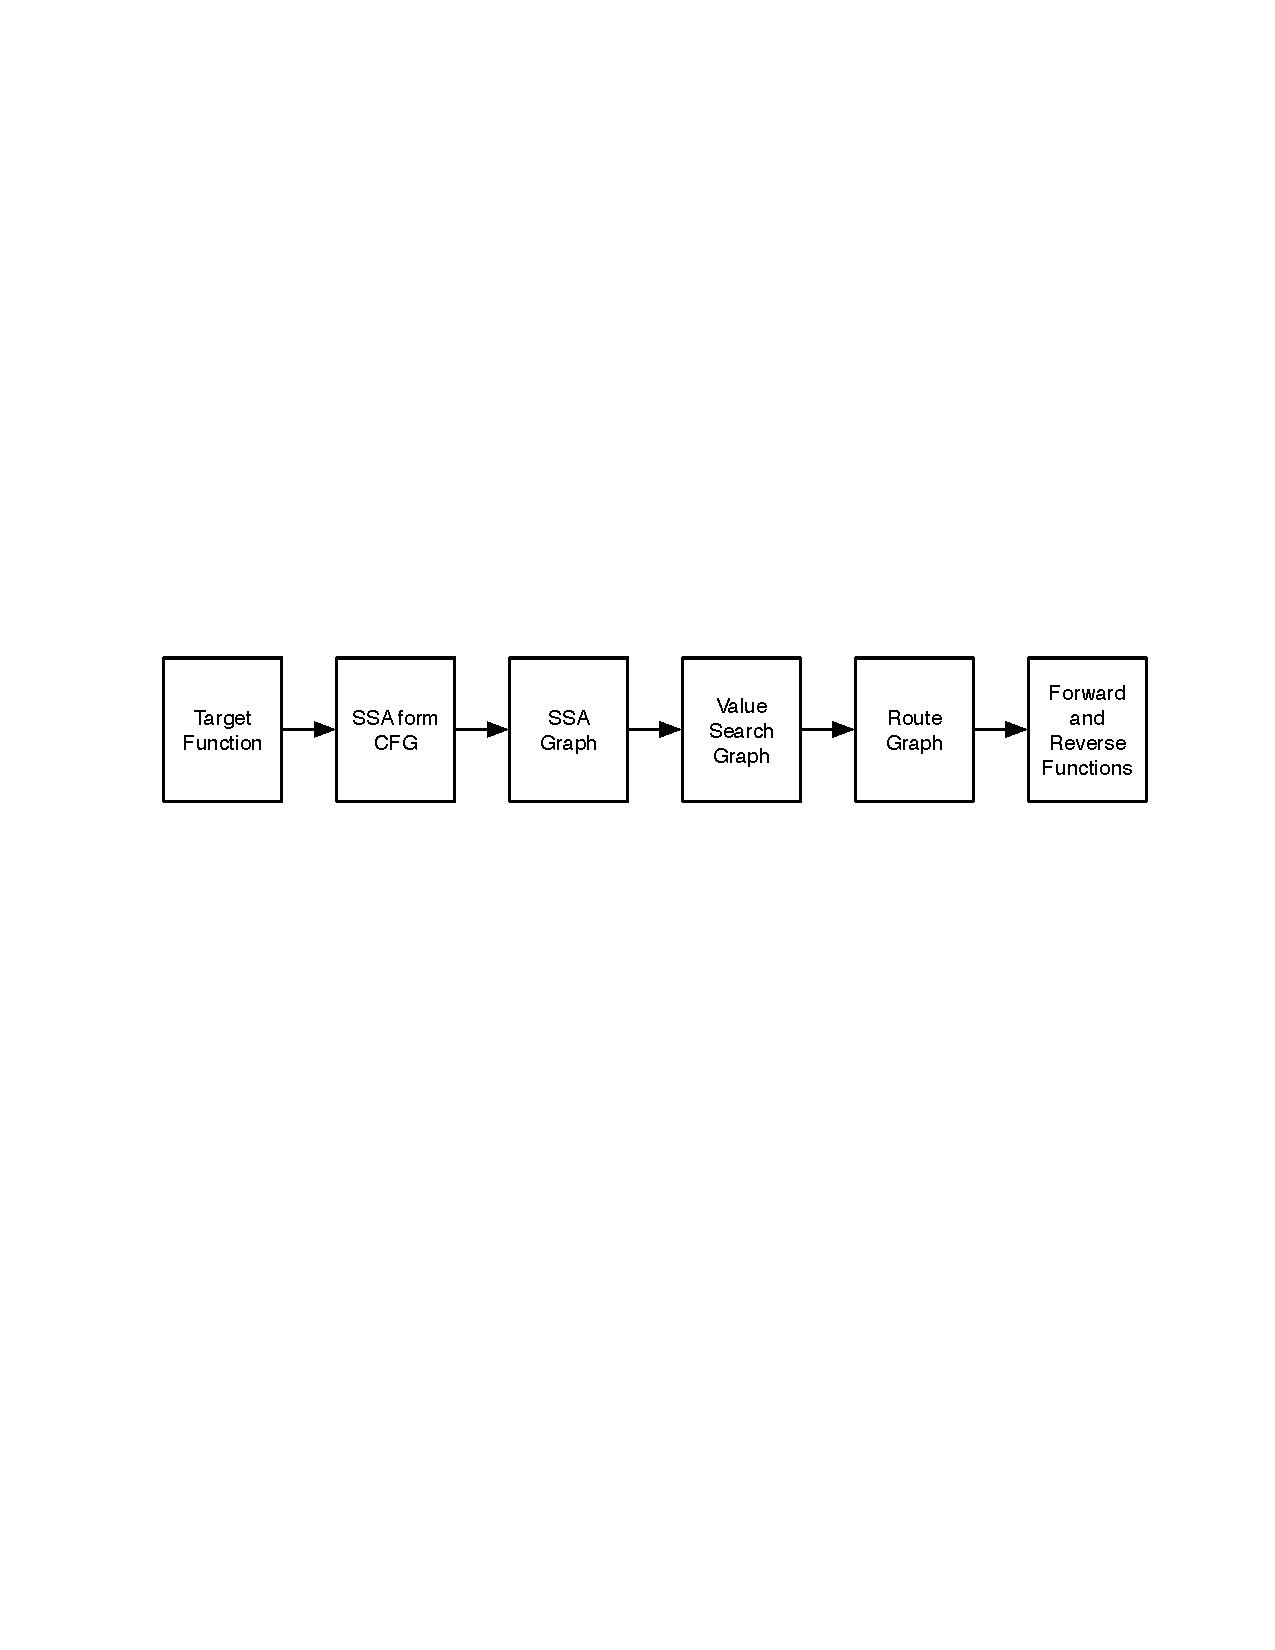
\includegraphics[width=400pt]{figures1/Framework.pdf}
\caption{Overall framework of the inversion algorithm}
\label{fig:framework}
\end{figure}

To restore target values, we will build a graph which shows equality relationships between values. 
We call this graph the \emph{value search graph}, and it is built based on an SSA graph \cite{Alpern1988,Cooper2001}. 
Then a search is performed on the value search graph to recursively find ways to recover the set of target values given the set of available values. 
If there is more that one way to restore a value, we choose the one with the smallest cost. 
The search result is a subgraph of the value search graph which we call a \emph{route graph}. 
For any path, a route graph shows a specific way to recover each target value from available values. 
Finally, the forward and reverse functions are built from a route graph. 
Figure \ref{fig:framework} illustrates this process.

In this section, we will use the example shown in Figure~\ref{fig:code_example} to illustrate our method.


\begin{figure}
\centering
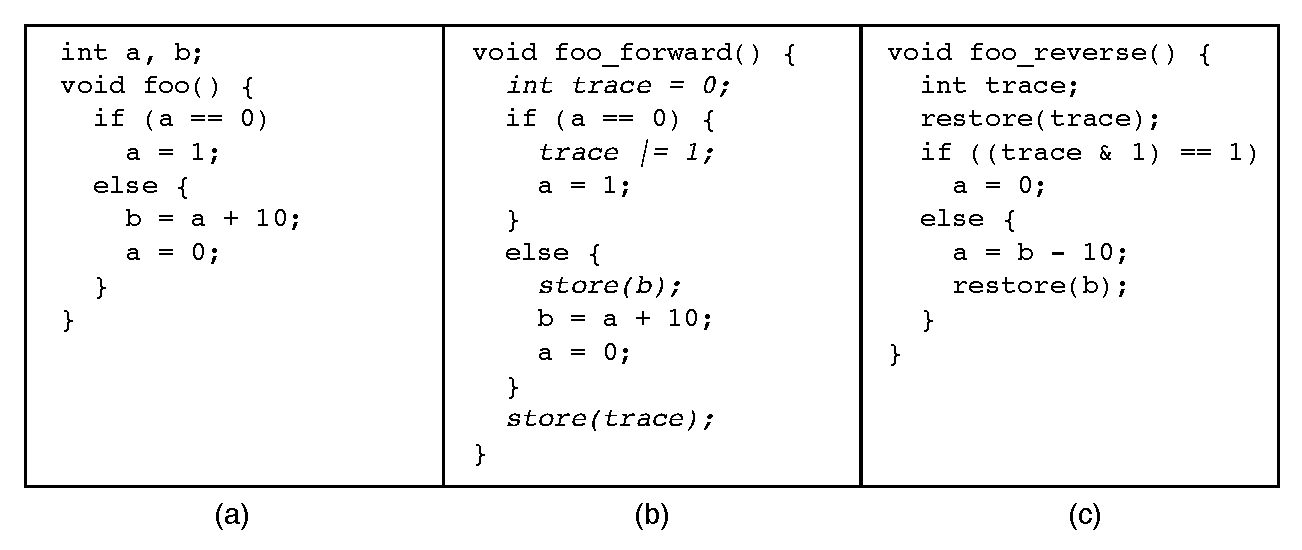
\includegraphics[width=400pt]{figures1/CodeExample.pdf}
\caption{(a) The original function $\quad$ (b) The forward function$\quad$ (c) The reverse function}
\label{fig:code_example}
\end{figure}

\subsection{The value search graph (VSG)}
We first build an SSA graph for the target function.
An SSA graph \cite{Alpern1988,Cooper2001}, built based on SSA form, consists of vertices representing operators, function symbols, or $\phi$ functions, and directed edges connecting uses to definitions of values. It shows data dependencies between different variables. 
The full algorithm for building an SSA graph is presented in \cite{Muchnick}. 
Figure \ref{fig:VSG}(a)(b) show the SSA-transformed CFG and its SSA graph for the function in Figure \ref{fig:code_example}(a). In this example, \texttt{a} and \texttt{b} are two target variables with initial values \texttt{a$_0$} and \texttt{b$_0$}, and final values \texttt{a$_3$} and \texttt{b$_2$}.

\begin{figure}
\centering
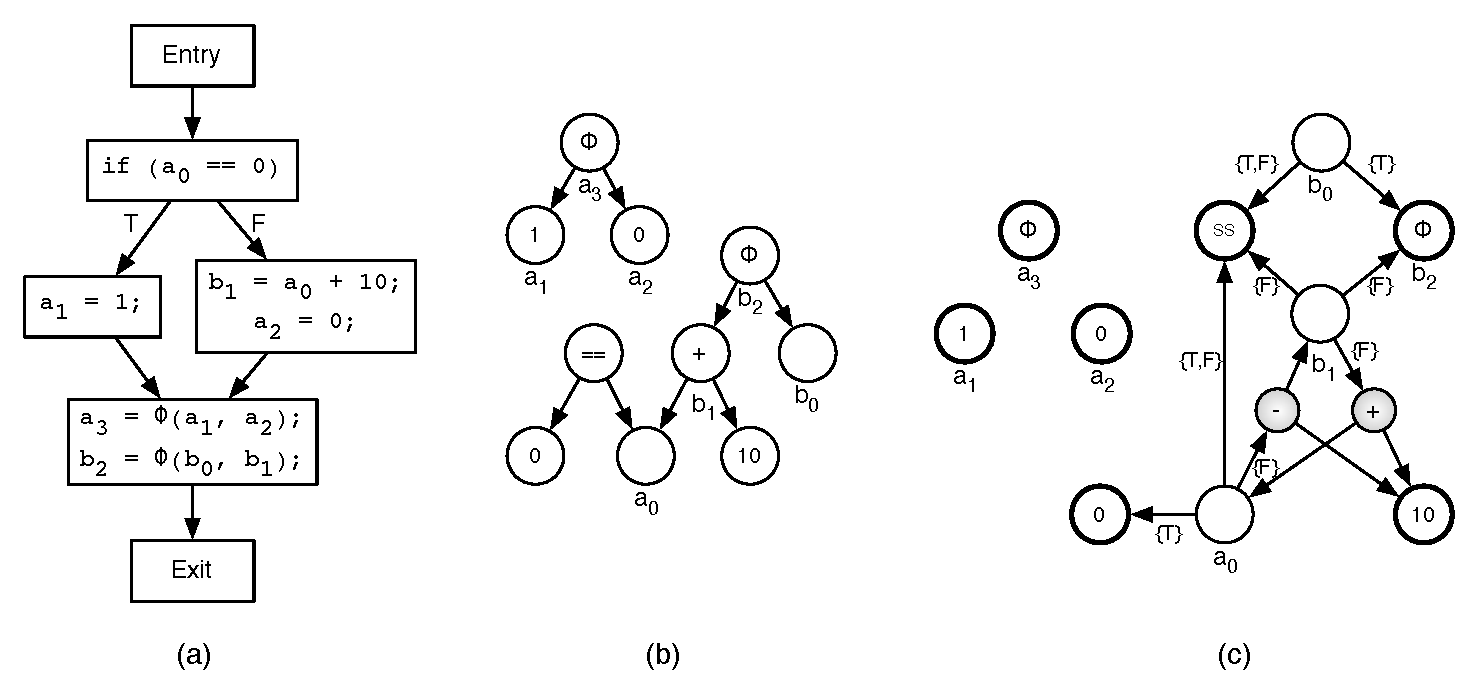
\includegraphics[width=400pt]{figures1/CFG.pdf}
\caption{(a) The SSA-transformed CFG of the function in Figure \ref{fig:code_example}(a)$\quad\quad$ (b) The corresponding SSA graph $\quad\quad$ (c) The corresponding value search graph. Nodes with bold outlines are available nodes; outgoing edges for these nodes are omitted because available nodes need not be recovered. `SS' is the special state saving node. Edges are annotated with their CFG path set.}
\label{fig:VSG}
\end{figure}




A \emph{value search graph} enables efficient recovery of values by explicitly representing equality relationships between values. 
Unlike an SSA graph, operation nodes are separated from value nodes in the value search graph, since their treatment is different for recovering values.
An edge connecting two value nodes $u$ and $v$ implies that $u$ and $v$ have the same value. 
%However, the equality of two values may only be true for certain CFG paths; hence each edge in a VSG is annotated with the set of CFG paths to which it applies.
An edge from value node $u$ to an operation node $op$ means that  $u$ is equal to the result of evaluating $op$ with its operands. 
To recover the value associated with node $v$, we can recursively search the graph starting at $v$.  

We attach a set of CFG paths to each edge in a value search graph, meaning the edge is applicable only if one of the CFG paths in that set is selected in the original function.
For operation nodes in the SSA graph, let the set of paths attached to each outgoing edge be the CFG paths for which the corresponding operation is executed. 
Similarly, for $\phi$ nodes, each reaching-definition edge should be annotated with all CFG paths for which the corresponding reaching definition reaches the $\phi$ function. 
We will describe an implementation of the path set representation later.

During the execution of the forward function, once a variable is assigned with a new value, its previous value may be destroyed and cannot be retrieved. To guarantee that a search in the value search graph can always restore a value, we introduce special \emph{state saving edges}. 
The idea behind these edges is that each value may be recovered by storing it during the forward execution. 
Whenever a state saving edge appears in the search results, the forward function is instrumented to save the corresponding value. 
The path set associated with a state saving edge for a value node $v$ is the set of all paths that include $v$'s definition. All state saving edges point to a unique \emph{state saving node}. %since it is not necessary to create a state saving node for every state saving edge.

\begin{comment}
\begin{figure}
\center{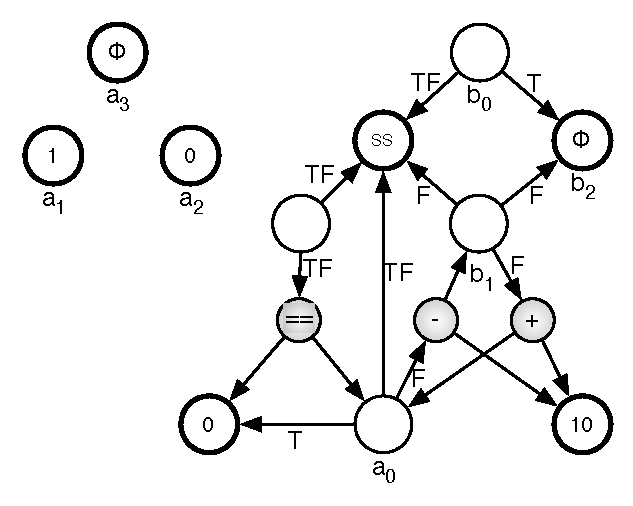
\includegraphics[width=160pt]{figures1/VSG.pdf}}
\caption{The value search graph for the function in Figure \ref{fig:code_example}(a). All available nodes are shown in bold. The label on edges from an operation node is only shown on the in-edge.}
\label{fig:VSG}
\end{figure}
\end{comment}

We apply the following rules to convert an SSA graph into a value search graph:
\begin{itemize}
	\item For simple assignment $v = w$, there is a directed edge from $v$ to $w$ in the SSA graph. 
	Since we can retrieve $w$ from $v$, add another directed edge from $w$ to $v$ with the same path set.

	\item A $\phi$ node in the SSA graph has several outgoing edges connecting all its possible definitions. 
	For each of those edges, add an opposite edge with the same path set. 
	
	\item For each operation node in the SSA graph, split it into an operation node and a value node, with an edge from the value node to the new operation node. 
	The new operation node takes over all outgoing edges, and the value node takes over all incoming edges. 
	
	\item If an equality operation (\texttt{==}) is used as a branching predicate and its outcome is true, we know that the two operands are equal.
	Therefore, we add edges from each operand to the other, with a path set for the edge equal to the path set of the \emph{true} CFG edge out of the branch. 
	We add the edges analogously for a not-equal operation (\texttt{!=}), but with the path set from the \emph{false} side of the branch.
	
	\item For every value that is not available, insert a state saving edge from the corresponding value node to the state saving node. 
\end{itemize}

\paragraph{Lossless operations} For certain operations, such as integer addition and exclusive-or, we can recover the value of an operand given the operation result and the other operand. For example, if $a=b+c$, we can recover $b$ given $a$ and $c$. For each such lossless operation, insert new operation nodes that connect its result to its operands, allowing the operands to be recovered from the result. The new nodes are added according to the following rules:
\begin{itemize}
	\item Negation (\texttt{a = -b}) and bitwise not (\texttt{a = \textasciitilde b}):$\;$ the new operations are  \texttt{b = -a} or \texttt{b = \textasciitilde a}, respectively.
	
	\item Increment (\texttt{++a}) and decrement (\texttt{--a}):$\;$ insert \texttt{--a} or \texttt{++a}, respectively.
	
	\item Integer addition (\texttt{a = b + c}) and subtraction:$\;$ for addition, the new operations are \texttt{b = a - c} and \texttt{c = a - b}; analogously for subtraction.
	
	\item Bitwise exclusive-or (\texttt{a = b \textasciicircum{ }c}):$\;$ insert \texttt{b = a \textasciicircum{ }c} and \texttt{c = a \textasciicircum{ }b}
\end{itemize}

\begin{comment}
\begin{figure}
\center{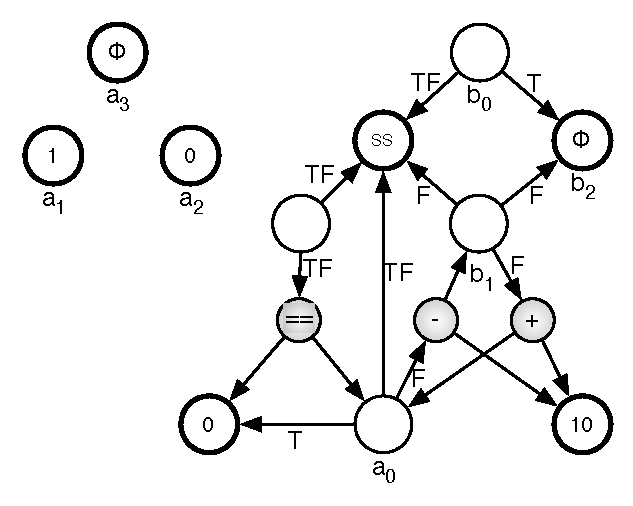
\includegraphics[width=160pt]{figures1/VSG.pdf}}
\caption{The value search graph for the function in Figure \ref{fig:code_example}(a). All available nodes are shown in bold. The label on edges from an operation node is only shown on the in-edge.}
\label{fig:VSG}
\end{figure}
\end{comment}

There are two special types of nodes in a value search graph: \emph{target nodes} are value nodes containing target values, and \emph{available nodes} are value nodes containing available values plus the state saving node.
As an optimization, we never create any outgoing edges for an available node. Figure \ref{fig:VSG}(c) shows the value search graph built for the code in Figure \ref{fig:code_example}(a). 
The available nodes are shown with a bold outline.
Since the function only has two paths, we use labels `T' and `F' to represent the CFG paths passing through the true and false body in the target function, respectively. 
The `--' operation node connecting $a_0$ to $b_1$ and the constant value `10' is generated from the `+' operation. 
The edge from $a_0$ to `0' for the path `T' is added based on the fact that $a_0 = 0$ on that path.
The `SS' node in the graph is the state saving node, and all unavailable nodes are connected to it. 
From the value search graph, we can find two valid ways to restore $b_0$ for the path `T': $b_0$ to SS node and $b_0$ to $b_2$. 
Obviously the second one is better since it avoids a state saving operation, and this better selection will be produced from the search algorithm described later.


\subsection{The route graph (RG)}
\label{sec:route-graph}

A \emph{route graph} is a subgraph of a value search graph connecting all target nodes to available nodes. Each route graph represents one way to restore the target values, and there may exist many valid route graphs for the same set of target values.
Edges in the route graph may have different path sets than the corresponding edges in the value search graph. 
For each edge $e$ in a route graph, let $P(e)$ denote the set of CFG paths that the edge is annotated with.
The following properties guarantee that the route graph properly restores all target values:

\begin{enumerate}[I)]

\item Let $\mathcal{U}$ be the set of all CFG paths. Then, for each target node $t$, 
	$$\bigcup_{\mathit{out} \in \text{OutEdges}(t)}P(\mathit{out}) \quad = \quad \mathcal{U} $$ 
	\label{rg-property-1}

\item For each node $n$ that is neither a target node nor an available node,
	$$\bigcup_{\mathit{out} \in \text{OutEdges} (n)} P(out) = \bigcup_{\mathit{in} \in \text{InEdges} (n)}P( \mathit{in} )$$ 

\item For each value node $n$, given any two outgoing edges $n\to p$ and $n\to q$, $P(n\to p) \cap P(n\to q) = \emptyset$ 

\item If $e$ is a route graph edge and its corresponding edge in the value search graph is $e'$, then $P(e) \subseteq P(e')$
	\label{rg-property-4}

\item For each directed cycle with edges $e_1 \dots e_n$,  $\quad \bigcap_{i=1}^n{P(e_{i})} = \emptyset$
	\label{rg-property-5}

\end{enumerate}

Property I specifies that each target value is recovered for every CFG path. 
Property II means that each value is recovered exactly for the paths for which it is needed.
Property III requires that for each CFG path, there is at most one way to recover a value. 
Property IV requires that the set of CFG paths associated with an edge in the route graph is a subset of the CFG paths originally associated with that edge in the value search graph. Finally, property V forbids self-dependence: restoring a value cannot require that value. 

\begin{figure}[htb]
\center{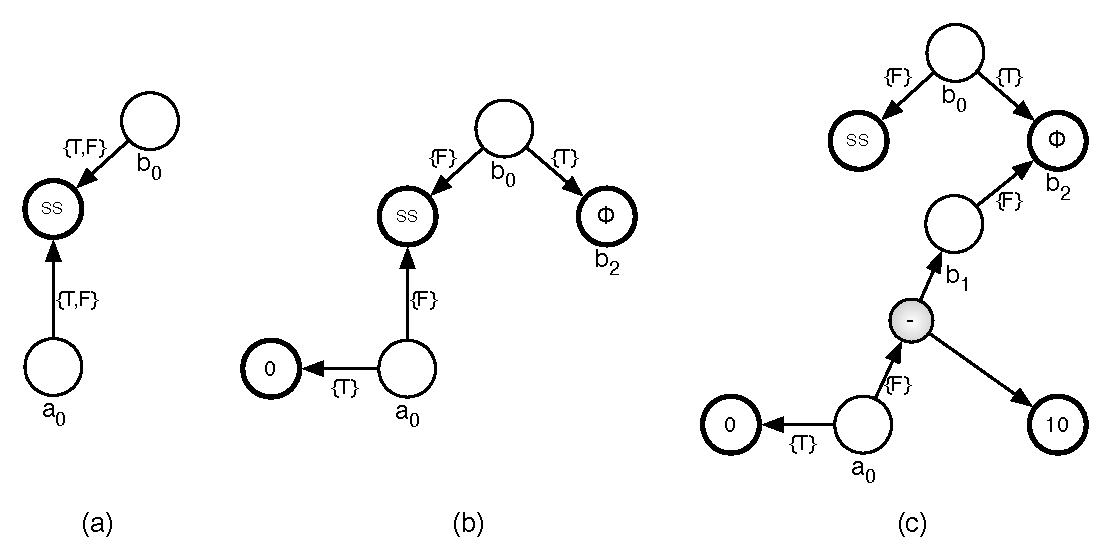
\includegraphics[width=400pt]{figures1/RG.pdf}}
\caption{Three different route graphs for the target values $\text{a}_{\text{0}}$ and $\text{b}_{\text{0}}$ given the the value search graph in Figure \ref{fig:VSG}(c). %While all three route graphs restore the target values, they have different costs.
}
\label{fig:RG}
\end{figure}

Figure \ref{fig:RG} shows three valid route graphs for the value search graph in Figure \ref{fig:VSG}. 
Route graph \ref{fig:RG}(a) only includes state saving edges. 
Route graph \ref{fig:RG}(b) takes advantage of the fact that for the `T' path the values of both \texttt{a$_0$} and \texttt{b$_0$} are known; it only uses staving for the `F' path. 
Route graph \ref{fig:RG}(c) improves upon route graph \ref{fig:RG}(b) by recomputing \texttt{a$_0$} as \texttt{b$_1$-10} for the CFG path `F'; state saving is only applied to \texttt{b$_0$} for path `F'.



\subsection{Searching the value search graph}

\subsubsection{Costs in route graphs}
As we have seen in Figure \ref{fig:RG}, there may be multiple valid route graphs that recover the target values, but with different overheads. 
In order to choose the route graph with the smallest overhead, we must define a cost metric.

Generally, there are two kinds of overhead in forward and reverse functions: execution speed and additional memory usage; we only consider the storage costs.
State saving contributes the most to the overhead memory usage and it also significantly affects the running time of both forward and reverse functions. 
Storing the path taken during forward execution is the other factor that contributes to memory usage; this overhead is bounded and is the same for all route graphs, so we exclude it from our cost estimate. 
With each state saving edge in the value search graph, we associate a cost equal to the size of the value that must be saved; other edges have cost 0.
%All other edges in the VSG have a small cost $\varepsilon$ associated with them, the technical reasons for which we will elucidate later. 
The cost of a route graph for a specific CFG path is the sum of the cost of those edges whose annotated path sets include that CFG path.

In Figure \ref{fig:RG}, suppose the cost to store and restore either \texttt{a} or \texttt{b} is $c$, the following table shows the cost of three route graphs for each CFG path.
% (here we ignore $\varepsilon$ just for clarity). 
Obviously the third route graph is the best one.

\begin{center}
\begin{tabular}{|c|c|c|c|}
%\begin{tabular}[c]{| c || m{1cm} | m{1cm} | m{1cm} |}
  \hline
  CFG path & route graph (a) & route graph (b) & route graph (c) \\
  \hline\hline
  T & $2c$ & $0$ & 0 \\
  \hline
  F & $2c$ & $2c$ & $c$ \\
  \hline
\end{tabular}
\end{center}

We have defined the cost of a single CFG path; however, a route graph may have different costs for different CFG paths.
When searching the value search graph, we would like to treat groups of CFG paths that share some edges in the route graph together, rather than performing a full search for each CFG path.
For this reason, the search algorithm partitions the CFG paths into disjoint sets of paths that have equal cost and we save the cost for each set of paths independently. 
In our search algorithm, we denote the costs of a route graph $r$ as $r.$costSet.
\[ r.\text{costSet} = \{ \langle P_{i}, c_{i} \rangle | P_{i}\text{ is a set of CFG paths and } c_{i} \text{ is the cost}\} \]
%\[P_{i} \cap P_{j} = \emptyset \quad \text{ if } i \neq j \]



\begin{algorithm}
\footnotesize
\label{algorithm:search}
\LinesNumbered
\DontPrintSemicolon

\SetKwData{NewCond}{newPaths}
\SetKwData{condition}{pathSet}
\SetKwData{cond}{paths}
\SetKwData{vertex}{target}
\SetKwData{edge}{edge}
\SetKwData{edges}{edges}
\SetKwData{edgeb}{e}
\SetKwData{target}{target}
\SetKwData{visited}{visited}
\SetKwData{subRoute}{newRoute}
\SetKwData{subGraph}{subGraph}
\SetKwData{route}{route}
\SetKwData{cost}{cost}
\SetKwData{eCopy}{eCopy}
\SetKwData{target}{target}
\SetKwData{subRoutes}{subRoutes}
\SetKwData{result}{resultRoute}
\SetKwData{costSet}{costSet}
\SetKwInOut{Input}{Initial input}

\SetKwFunction{OutEdges}{OutEdges}
\SetKwFunction{SearchSubRoute}{SearchSubRoute}
\SetKwFunction{SearchRoute}{SearchRoute}
\SetKwFunction{UpdateConditions}{ChooseMinimalCosts}

\Input{The search start point \vertex, with \cond $= \emptyset$, \visited $= \emptyset$}




\BlankLine
\SearchSubRoute{\vertex, \cond, \visited} \;
\Begin{
  \result $\leftarrow \emptyset$,  \subRoutes $\leftarrow \emptyset$ \;
  \If{\vertex is an operation node}{
      \ForEach{\edge $\in$ \OutEdges{\vertex}}{
          \lIf{\edge.\target $\in$ \visited}{\Return $\emptyset$\;}
          \subRoute $\leftarrow$ \SearchSubRoute{\edge.\target, \cond, \visited}\; 
          \lIf{\subRoute $= \emptyset$}{\Return $\emptyset$\;}
          add \edge and \subRoute to \result \;
      }
      \Return \result \;
  }
  \If{\vertex \mbox{is available}}{
      add \vertex to \result \;
      add $\langle \cond, 0 \rangle$ to \result.\costSet \;
      \Return \result \;
  }
  \ForEach{\edge $\in$ \OutEdges{\vertex}}{
    \lIf{\edge.\target $\in$ \visited}{continue}  
    \BlankLine
    \NewCond $\leftarrow$ \edge.\condition $\cap$ \cond\; 
    \lIf{\NewCond $=  \; \emptyset$}{continue} 
    \BlankLine

    \subRoute $\leftarrow$ \SearchSubRoute{\edge.\target, \NewCond, \visited$\cup \; \{\vertex\}$}\;
 
    add \edge with paths \NewCond to \subRoute\;
    \lForEach{$\langle \cond, \cost \rangle$ in $\subRoute.\costSet$}{
        \cost += \edge.\cost\;
    }
        \lForEach{\route in \subRoutes}{
    \UpdateConditions{\route, \subRoute}\;
    }


      add \subRoute to \subRoutes \;

  }
  add \vertex to \result \;
  \ForEach{\route in \subRoutes}{
      \lIf{$\route.\condition \ne \emptyset$}{
          add \route to \result \;
      }
  }
  \Return \result \;
}

\SetKwData{routea}{route1}
\SetKwData{condition}{pathSet}
\SetKwData{routeb}{route2}
\SetKwData{edge}{edge}
\SetKwData{graph}{routeGraph}
\SetKwData{conda}{paths1}
\SetKwData{condb}{paths2}
\SetKwData{costa}{cost1}
\SetKwData{costb}{cost2}
\SetKwData{paths}{paths}
\SetKwData{cost}{cost}

\BlankLine
\BlankLine
\UpdateConditions{\routea, \routeb} \;
\Begin{
    \lIf{\routea.\condition $\cap$ \routeb.\condition  $ = \emptyset$}{
        return\;
    }
    \ForEach{$\langle \conda, \costa \rangle$ in \routea.\costSet}{
        \ForEach{$\langle \condb, \costb \rangle$ in \routeb.\costSet}{
            \lIf{\conda $\cap$ \condb $= \emptyset$}{
                continue\;
            }
            \If{\costa $>$ \costb} {$\conda \leftarrow \conda - \condb $\;
            Remove (\conda $\cap$ \condb) from all edges of \routea \;}
            \Else{$\condb \leftarrow \condb - \conda $\;
            Remove (\conda $\cap$ \condb) from all edges of \routeb \;}
        }
    }
    \routea.\condition $ = \bigcup_{\langle \paths, \cost \rangle \in \routea.\costSet} \paths $ \;
    \routeb.\condition $ = \bigcup_{\langle \paths, \cost \rangle \in \routeb.\costSet} \paths $
}

\caption{Searching for a route graph in a value search graph}

\end{algorithm}

\subsubsection{Search algorithm}
Our search algorithm should aim to find a route graph that has the minimum cost for each path. 
Theoretically, however, searching for a minimal route graph is an NP-complete problem. 
To make the problem tractable, we apply the heuristic of finding a route graph for each target value individually; the individual route graphs are then merged into a route graph that restores all the target values. 
Similarly, in order to recover the value of a binary operation node, we recover each of the two operands independently and then combine the results. 

The pseudocode for our heuristic search algorithm is presented in Algorithm \ref{algorithm:search}. 
The {\tt SearchSubRoute} function returns a route graph given a target node, the paths for which that node must be restored, and the set of value nodes visited so far.
The algorithm explores all ways to recover the current node by calling itself recursively on all the nodes that are directly reachable from the current node; available nodes are the base case.
Lines 5--10 handle recovering the values of operation nodes. 
In order to recover the value of an operation node, each of its operands must be recovered.
Lines 11--14 return a trivial route graph for available nodes, with a cost of 0. 
The remaining body of the algorithm (lines 15--27) handles recovering a value node that is not available.
Each of the out-edges of the target node may be used to recover its value for the CFG paths associated with that edge; these edges are explored in the {\tt for}-loop in lines 15--23.
The variable {\tt newPaths} on line 17 represents the set of paths that we are both interested in and are associated with the current edge. 
In line 19, we recursively find a route graph that recovers the target value by recovering the target of the current outgoing edge.
Lines 21--22 update the cost sets of the new route graph; if it provides a lower cost for some CFG path than the solutions found so far, the partial results are modified so that each CFG path is restored with the cheapest route graph.
Finally, the route graph from line 19 is added to the list of partial results (line 23). 
After all out-edges of the target node have been explored, the partial results are merged into a single route graph and returned (lines 24--27).
Note that it is unnecessary to check whether the target node has been successfully recovered, since the state saving edge always provides a valid route graph for the node. 
Figure \ref{fig:RG}(c) shows the route graph produced by the algorithm when searching the value search graph from Figure \ref{fig:VSG}(c).

The search algorithm enforces properties \ref{rg-property-1}--\ref{rg-property-4} from section \ref{sec:route-graph} during its execution.
To make sure that the search result does not contain cycles (property \ref{rg-property-5}), we record which value nodes are already in the route using a set \texttt{visited} in Algorithm \ref{algorithm:search}. 
This alone is not sufficient to guarantee that the result is acyclic, for there may be two different paths with identical cost to recover a single value node. 
If one way is chosen to recover a value node $v$ during path of the search, and then later $v$ is recovered differently for the same CFG path, a cycle may form.
To prevent this situation from occurring, we always traverse out-edges in the same order of line 19 of Algorithm \ref{algorithm:search}; the first route graph with the smallest cost is chosen. In addition, two paths coming from two different value nodes may also form a cycle when all costs on edges of the cycle are 0. We eliminate this possibility by replacing 0 by a small cost $\varepsilon$.
% Do we really need to have epsilon for correctness? It seems that the above condition is sufficient to guarantee correctness

\begin{comment}
\paragraph{Extensions} Adding constraints during the search could produce different inversion strategies. 
For example, putting only state saving edges to the route graph will produce the same result as checkpointing.
Including state saving edges and phi edges (edges incident to a phi node) results in the incremental state saving, where a variable is saved only for the paths for which it is modified. 
\end{comment}

\subsection{Instrumentation and Code generation}

\subsubsection{Representing CFG path sets}

Our search algorithm relies on efficiently computing intersection, union, and complement of CFG path sets, as well as testing whether the set of paths is empty; for this reason we suggest implementing the set representations as bit vectors. 
Ball and Larus \cite{Ball1996} present an path profiling method in which each path is given a number from 0 to $m-1$, where $m$ is the count of the CFG paths. 
We use their algorithm to number each path, and for each path we associate exactly one bit in the bit vector used to represent a path set.
%Algorithm \ref{algorithm:findPaths} illustrates how to use depth-first search on the CFG to find the set of paths that correspond to each CFG edge; the search is initially invoked with \texttt{FindCfgPaths(Entry, 0)}.

\begin{comment}

\begin{algorithm}
\label{algorithm:findPaths}
\DontPrintSemicolon
\caption{Finding the set of paths passing through each CFG edge}



\SetKwFunction{findCfgPaths}{FindCfgPaths}
\SetKwFunction{OutEdges}{OutEdges}

\SetKwData{node}{node}
\SetKwData{edge}{edge}
\SetKwData{target}{target}
\SetKwData{pathIndex}{pathIndex}
\SetKwData{exitNode}{\textbf{Exit}}
\SetKwData{pathsHere}{pathsFound}
\SetKwData{pCount}{count}

\BlankLine
\findCfgPaths{\node, \pathIndex} \;
\Begin{
	\lIf{\node == \exitNode}
	{
		\Return 1 \;
	}
	\pathsHere $\leftarrow$ 0 \;

	\ForEach{\edge $\in$ \OutEdges{\node}}
	{
		\pCount $\leftarrow$ \findCfgPaths{\edge.\target, \pathIndex} \;
		Add paths \pathIndex through (\pathIndex + $\pCount - 1$) to \edge \;
		\pathsHere $\leftarrow$ \pathsHere + \pCount \;
		\pathIndex $\leftarrow$ \pathIndex + \pCount \;
	}
	\Return{\pathsHere} \;
}

\end{algorithm}

\end{comment}

\subsubsection{Recording CFG paths}
\label{sec:encoding-paths}
\begin{comment}
We can encode a path with a path number as above, and checking if a path set represented by a bit vector contains a path is also fast. However, the length of a bit vector equals the number of CFG paths, which can be large. Further, we will see later that each branch in the reverse function is translated from the path set on a route graph edge. If there are $m$ CFG paths in the target function, and $n$ distinct path sets used to generate the predicates in the reverse function, then we need $m\times n$ bits of static memory in the reverse function! %Another problem comes that we may also need the condition  in the forward method for the state saving statement. 
Our solution is using another method to encode CFG paths. We will see that a path set can be transformed to a set of new representations, from which we can build more efficient predicates in the reverse function.
\end{comment}

We need to store path information in a way that allows us to efficiently record the CFG path taken (for forward execution), and to efficiently check if the path matches a given set of CFG paths attached to a route graph edge (for reverse execution). 
However, if we encode each path using its path number, then examining whether a path is a member of a set is inefficient.
% (we don't want each path set represented by a bit vector to appear in the reverse code, which may take too much memory). 
Instead we  %employ another approach to encoding paths, and 
use a bit vector to record the CFG path, in which each bit represents the outcome of a branching statement. 
%We will see later that this new path encoding will result in quite efficient comparisons in the reverse execution.
Since this method is similar to \emph{bit tracing}\cite{Ball1994}, we call this bit vector a \emph{trace}.
Note that two branches may share the same bit if they cannot appear in the same path. Thus, the number of bits required to store the path taken is equal to the largest number of branches that appear on a single CFG path.
Algorithm \ref{algorithm:conditions} calculates bit-vector position for each branch node accordingly.

\begin{algorithm}
\label{algorithm:conditions}
\DontPrintSemicolon

\SetKwData{vertex}{u}
\SetKwData{vertexa}{v}
\SetKwData{vertexb}{w}
\SetKwData{mask}{mask}
\SetKwFunction{bitPosition}{position}
\SetKwFunction{maxVal}{max}

\BlankLine
\BlankLine
    \ForEach{CFG node \vertex in reverse topological order}{
        \uIf{\vertex is a leaf node}{
            \bitPosition{\vertex} $\leftarrow$ -1 \;
        }
            \uElseIf{\vertex is a branch node}{
                \tcc{$\vertex\to\vertexa$ and $\vertex\to\vertexb$ are its two out-going edges} 
                \bitPosition{\vertex} $\leftarrow$ \maxVal{\bitPosition{\vertexa}, \bitPosition{\vertexb}} + 1\;
            }
            \Else{ 
                \tcc{$\vertex\to\vertexa$ is its out-going edge} 
                \bitPosition{\vertex} $\leftarrow$ \bitPosition{\vertexa} \;
            }         
    }

\caption{Generating the bit position for each branch node.}
\end{algorithm}

In the forward function, we use an integer as the bit vector to record all predicate results\footnote{Potentially we could omit recording predicates that do not affect the reverse function.}. 
Let \texttt{trace} be the variable recording a trace, initialized to zero; then the true edge of each branch node $v$ is instrumented with the statement \footnote{We use several operators in C/C++ syntax here and below, which includes bitwise OR operator \texttt{|}, bitwise AND operator \texttt{\&}, bitwise left shift operator  \texttt{<<}, equal to operator \texttt{==}, and logical OR operator \texttt{||} .}
$$ \texttt{trace = trace  | (1 << $\mathit{position(v)}$)}; $$ 
where $\mathit{position(v)}$ is calculated by Algorithm \ref{algorithm:conditions}. 
The variable \texttt{trace} is stored at the end of the forward function and restored at the beginning of the reverse function. 
Note that we can further optimize the instrumentation by moving a trace updating operations downward through the CFG and merging them.
%The Ball and Larus maximal spanning tree method for calculating edges to instrument is also applicable \cite{Ball1996}. 



In the reverse function, we must test if \texttt{trace} matches the path sets that appear on route graph edges. We start with transforming each path in the set into a trace (the trace for each path can be computed by the same means as recording a trace in the forward function).
Then, checking if a path set contains a path represented by \texttt{trace} is done by comparing it to each trace. 
Suppose a path set containing two paths is transformed into two traces \texttt{01101} and \texttt{01001}. Instead of comparing \texttt{trace} to each of them as:
$$ \texttt{if (trace == 01101 || trace == 01001)} $$ 
we can simplify this predicate by using a mask \texttt{11011} on \texttt{trace}:
$$ \texttt{if ((trace \& 11011) == 01001)} $$ 

The combined trace for \texttt{01101} and \texttt{01001} is \texttt{01$\times$01}, where $\times$ denotes that the bit does not matter. 
Given a set of traces, we can combine pairs repeatedly to reduce the size of the set.
This greatly reduces the complexity of the branching statements in the reverse code. 
\begin{comment}

Each CFG path is induced by a sequence of branches that must be either true or false; we can build the corresponding mask by setting 0 or 1 in the position corresponding to each branch. 
Some elements of the mask representing a CFG path may be $\times$, which signifies that the outcome of the corresponding branch does not affect whether the path is taken or not. 
Algorithm \ref{algorithm:computeMasks} computes the path mask associated with each CFG path; it is initially invoked as \texttt{ComputePathMasks(Entry, 0, $\times$$\times$$\dots$$\times$$\times$)}. 
Note that the indices computed for each path by Algorithm \ref{algorithm:computeMasks} match those computed by Algorithm \ref{algorithm:findPaths}; in fact, these two algorithms can be merged into one. 


\begin{algorithm}
\label{algorithm:computeMasks}
\DontPrintSemicolon
\caption{Finding mask corresponding to each CFG path}

\SetKwFunction{computePathMasks}{ComputePathMasks}
\SetKwFunction{OutEdges}{OutEdges}

\SetKwData{node}{node}
\SetKwData{edge}{edge}
\SetKwData{target}{target}
\SetKwData{pathIndex}{pathIndex}
\SetKwArray{currentMask}{currentMask}
\SetKwData{exitNode}{\textbf{Exit}}
\SetKwData{pathsHere}{pathsFound}
\SetKwData{pCount}{count}
\SetKwFunction{bitPosition}{position}
\SetKwData{edgeLabel}{label}

\BlankLine
\computePathMasks{\node, \pathIndex, \currentMask} \;
\Begin{
	\If{\node = \exitNode}
	{
		\currentMask is the mask for the path \pathIndex \;
		\Return 1
	}
	\pathsHere $\leftarrow$ 0 \;

	\ForEach{\edge $\in$ \OutEdges{\node}}
	{
		\If{\edge is labeled} 
		{
			\currentMask{\bitPosition{\node}} $\leftarrow$ 
			$\begin{cases} 0 \text{ if } \edge.\edgeLabel = F \\ 1 \text{ if } \edge.\edgeLabel = T \end{cases}$
		}
		\pCount $\leftarrow$ \computePathMasks{\edge.\target, \pathIndex, \currentMask} \;
		\pathsHere $\leftarrow$ \pathsHere + \pCount \;
		\pathIndex $\leftarrow$ \pathIndex + \pCount \;
	}
	\Return{\pathsHere} \;
}

\end{algorithm}

In order to test the recorded path against a set of CFG paths, we may test the mask of the path against each of the masks in the set. 
For example, we can test for the mask 00$\times$10 with \texttt{((cfgmask \& 11011) == 00010)}.
To make these checks more efficient, however, we may merge multiple CFG paths into a single mask.
For example, if the masks for two paths are $0011$ and $0111$, we can test for either path with the mask 0$\times$11. 

\end{comment}


Algorithm \ref{algorithm:mergeMasks} starts out with all traces corresponding to a set of CFG paths and merges them into a minimal set of traces that can be used to test membership in the set. 
The intuition behind Algorithm \ref{algorithm:mergeMasks} is that if the traces are sorted so that bit $i$ is the least significant bit, the traces that are identical to each other except for bit $i$ will be adjacent. 
However, if we are careful we don't have to pay the full sorting cost for each bit $i$. 
If the traces are sorted when their bits are considered in the order $b_{1} b_{2} \dots b_{i - 1} \quad b_{k} b_{k - 1} \dots b_{i} $ and we want to sort them according to the bit order $b_{1} b_{2} \dots b_{i - 2} \quad b_{k} b_{k - 1} \dots b_{i - 1} $, we need only sort each sequence of the trace for which bits 1 through $(i-2)$ are identical. 
For each such sequence, there are at most three sorted subsequences, indexed by bit $b_{i-1}$; these can be merged in linear time (similarly to mergesort).
If we use a linear-time sort, such as radix sort, for the first iteration, the overall runtime of Algorithm \ref{algorithm:mergeMasks} is $O(k n)$, where $n$ is the size of the path set.


\begin{algorithm}
\label{algorithm:mergeMasks}
\DontPrintSemicolon
\caption{Merging a set of path traces}

\SetKwFunction{mergePathMasks}{MergePathTraces}

\SetKwArray{masks}{traces}
\SetKwData{bitSize}{k}
\SetKwData{index}{i}
\SetKwData{maskIndex}{j}

\SetKw{KwDownTo}{down to}

\SetKwFunction{length}{Length}

\mergePathMasks{\masks} \;
\Begin{
	\tcc{Each trace has \bitSize "bits", and each bit is 0, 1, or $\times$}
	\tcc{Bits are numbered ascendingly; e.g. $m = b_{1} b_{2} \dots b_{k}$}

	\For{\index $\leftarrow$ \bitSize \KwDownTo $1$}
	{
		\tcc{Note: for \index = k, the bit ordering is $m = b_{1} b_{2} \dots b_{k}$}
		Sort \masks, where trace bits are ordered $b_{1} b_{2} \dots b_{i - 1} \quad b_{k} b_{k - 1} \dots b_{i} $ \;
		
		\For{\maskIndex $\leftarrow$ 2 \KwTo \length{\masks}}
		{
			\If{ \masks{\maskIndex$-\;1$} and \masks{\maskIndex} match except for bit \index}
			{
				set bit \index to $\times$ for  \masks{\maskIndex$-\;1$} \;
				delete \masks{\maskIndex}
			}
		}
	}
	

	
}

\end{algorithm}

After the merge, if we have $n$ traces $t_1,...,t_n$ for a path set, the resulting predicate would be:
$$\texttt{if ((trace \& $mask_1$) == $obj_i$ || ... || (trace \& $mask_n$) == $obj_n)$}$$
For each trace $t_i$, $mask_i$ is obtained by setting all bits which are $\times$ in $t_i$ to 0 and others to 1, and $obj_i$ equals $mask_i$ \texttt{\&} $t_i$.



\subsubsection{Inserting state saving statements}
\label{sec:state-saving}
The other instrumentation in the forward function are state saving statements, which are inserted according to the state saving edges in the route graph. 
For each state saving edge in the route graph, suppose the variable to store is $var$ and the path set on this edge is $P$. 
Our task is finding one or several locations to store $var$ according to the path set $P$, ensuring that $var$ is only saved once for each CFG path in $P$. 

To find such locations, we first compute the corresponding path traces $T$ of $P$ from Algorithm \ref{algorithm:mergeMasks}. 
For each trace in $T$, we traverse the CFG from the entry. 
When we reach a branch node, check the corresponding bit in the trace: fall through the true edge if the bit is 1, false edge if the bit is 0. 
If the bit is $\times$, the traversal forks and that bit is assigned to 0 and 1 respectively forming two new traces; and for each concretized trace the descent continues. 
The descent stops immediately when all bits which are not checked in the trace are $\times$. 
After this process, we obtain one or more locations where the descent has stopped. 
%This is not clear. It's better to leave it out than to have it be confusing
%If the tracings from two traces stop at the same location, we then combine them again (since they may be forked from one trace previously). 
%In each maximal basic block in which each location resides, 
In each location we find a point where the definition of $var$ is reachable and a state saving statement is inserted there. 
However, it is possible that the path set containing the paths passing through this location is larger than the one on which the state saving is needed. 
In this case, we guard the state saving statement with a branch whose predicate corresponds to the trace at this location.



\subsubsection{Building a CFG for the reverse function}
We build the CFG for the reverse function from a route graph; the reverse CFG is acyclic and each path in it must obey the data dependencies represented in the route graph.
Each outgoing edge from a value node in the route graph will be translated to a statement in the reverse function. 

There could be a large number of correct reverse CFGs for a route graph, resulting in different control flows and different numbers of branches. 
%Without the runtime information such as profiling data, it is difficult to determine with one is the best with respect to the performance. 
We choose to build a structured CFG to simplify the translation to source code. 
We also attempt to minimize the number of predicates in the CFG. 

There are three kinds of statements that can be generated from a route graph:
\begin{itemize}
	\item An operator node with its operands and result induces an operation statement,  such as \texttt{a = b + c}.
	\item An edge with value nodes as both ends induces an assignment statement.
	\item An edge pointing to the SS node induces an value restoration statement.
\end{itemize}

%For the purposes of code generation, we shall refer to an operation node together with its incoming and outgoing edges as an operation (hyper)edge, which is a special edge with one source and one or more targets.
%With this convention, each statement corresponds to one ``edge'' in the route graph.

The statements generated from route graph edges retain the path sets attached to the corresponding edges.
We build basic blocks of statements that all share the same path sets, and insert branches so that each basic block is executed when the corresponding path is taken in the forward function. 
While enforcing the path set constraints ensures correct control flow, producing correct data flows depends on the order in which statements are inserted in the CFG.
Note that a route graph corresponds to explicit data dependencies, and for each CFG path in the forward function it is acyclic due to property \ref{rg-property-5} from section \ref{sec:route-graph}. 
Hence, if we order statements in the reverse topological order of the route graph edges, dataflow dependencies are correctly maintained.

\begin{algorithm}
\footnotesize
\label{algorithm:reverse-cfg}
\LinesNumbered
\DontPrintSemicolon
\caption{Generating a CFG for the reverse function from a route graph.}


\SetKwData{bb}{b}
\SetKwData{bone}{b1}
\SetKwData{btwo}{b2}
\SetKwData{stmts}{pendingStmts}
\SetKwData{bbs}{openBlocks}
\SetKwData{s}{s}
\SetKwData{cond}{pathSet}
\SetKwData{cp}{pathSetPairs}
\SetKwData{edge}{edge}
\SetKwData{valNode}{valNode}
\SetKwData{RG}{routeGraph}
\SetKwData{CFG}{cfg}
\SetKwData{source}{source}
\SetKwData{availNode}{availNode}
\SetKwFunction{GenerateReverseCFG}{GenerateReverseCFG}
\SetKwFunction{GetStatements}{BuildReadyStatements}
\SetKwFunction{InEdges}{InEdges}

\SetKwFunction{BuildBB}{BuildBasicBlock}
\SetKwData{entry}{entry}

\BlankLine
\GenerateReverseCFG{\RG}\\
\Begin
{
	\CFG $\leftarrow \emptyset$, \stmts $\leftarrow \emptyset$, \bbs $\leftarrow \emptyset$, \cp $\leftarrow \emptyset$\; 
	\lForEach{\valNode in \RG}
	{
		\valNode.\cond $\leftarrow \emptyset$\;
	}
	\ForEach {available node \availNode in \RG}
	{
		\GetStatements{\availNode, $\mathcal{U}$, \stmts} \;
	}
	\CFG.\entry $\leftarrow$ \BuildBB{$\mathcal{U}$} \;
	%Create a new basic block with path set $\mathcal{U}$ as the entry of the CFG and add it to \CFG and \bbs\;
    
	\While{$\stmts \neq \emptyset$}
	{
		\uIf{$\exists \s \in \stmts, \bb \in \bbs$, and $\s.\cond = \bb.\cond$}
		{
			Append \s to \bb\;
			\valNode $\leftarrow$ the source node of the edge that generated \s \;
			 \GetStatements{\valNode, \s.\cond, \stmts}\;
 		}
		\uElseIf{$\exists \s \in \stmts, \bb \in \bbs$, and \s.\cond $\subset$ \bb.\cond}
		{
			Append to \bb a branch, with the predicate generated from \s.\cond\;
			\bone $\leftarrow$ \BuildBB{\s.\cond} \;
			Append \s to \bone\;
			\btwo $\leftarrow$ \BuildBB{$\bb.\cond - \s.\cond$} \;
			%Create two new basic blocks $\bone$ and $\btwo$ with path set \s.\cond and $\bb.\cond - \s.\cond$ respectively, and add them to \CFG and \bbs\;
			Insert into \CFG edges from \bb to \bone and \btwo with labels \textit{true} and \textit{false} \;
			Add $\langle \bone.\cond, \btwo.\cond \rangle$ to \cp\;
			\bbs $\leftarrow \; \bbs - \{ \bb \}$ \;
			%Remove  \bb from \bbs\;
			\valNode $\leftarrow$ the source node of the edge that generated \s \;
			\GetStatements{\valNode, \s.\cond, \stmts}\;
 		}
		\ElseIf{$\exists \bone, \btwo \in \bbs$, and $\langle \bone.\cond, \btwo.\cond \rangle \in \cp$}
		{
			\bb $\leftarrow$ \BuildBB{\bone.\cond $\cup$ \btwo.\cond} \;
			%Create basic block \bb, $\bb.\cond = \bone.\cond \cup \btwo.\cond$, and add \bb to \CFG and \bbs\;
			Insert into \CFG two edges, from \bone and \btwo to \bb\;
			\cp $\leftarrow \; \cp - \{ \langle \bone.\cond, \btwo.\cond \rangle \}$ \;
			%Remove $\langle \bone.\cond, \btwo.\cond \rangle$ from $\cp$\;
			\bbs $\leftarrow \; \bbs - \{ \bone, \btwo \}$ \;
			%Remove \bone and \btwo from \bbs\;
			\lIf{$|\bbs| = 1$}{break}
		}
	}
	\Return{\CFG}
}

\BlankLine

\SetKwData{availablePathSets}{nodeAvailablePaths}

\GetStatements{\valNode, \availablePathSets, \stmts}\\
\Begin
{
	\valNode.\cond $\leftarrow$ \valNode.\cond $\cup$ \availablePathSets \;
	\ForEach{\edge $\in$  \InEdges{\valNode}}
	{
		\If{\edge.\cond $\subseteq$ \valNode.\cond}
		{
			\uIf{\edge.\source is an operation node}
			{
				Set \edge to be a available for \edge.\source \;
				\If{all operands of \edge.\source are available}
				{
					Add to \stmts the statement for for \edge.\source, with path set \edge.\cond \;
				}
			}
		\Else
		{
			Add to \stmts the statement for \edge, with path set \edge.\cond \;
		}}
	}
}
\BlankLine

\BuildBB{\cond}
\Begin
{
	Build an empty basic block \bb and attach path sets \cond to it. \;
	\CFG $\leftarrow$ \CFG $\cup$ \{ \bb \}, $\quad$
	\bbs $\leftarrow$ \bbs $\cup$ \{ \bb \} \;
	\Return{ \bb } \;
}

\end{algorithm}

Algorithm \ref{algorithm:reverse-cfg} shows how to build a CFG for the reverse function. 
We keep a set of basic blocks, \texttt{openBlocks}, to which new statements can be appended.  
We also maintain a set of statements, \texttt{pendingStmts}, whose data dependencies have been satisfied, but which have not yet been inserted in the CFG.
Each basic block has an associated path set; these are the paths in the forward function for which the corresponding basic block in the reverse function should execute.
Similarly, each statement has a set of paths from the forward function. 
If there is a pending statement and an open basic block whose path sets match, we simply append the statement to the basic block.
When a statement is inserted into the CFG, the data dependencies of new statements may now be satisfied; we call the function \texttt{BuildReadyStatements} to generate the statements that are now valid for insertion. 
If there is no pending statement whose path set matches the path set of an open basic block, we must insert or join a branch in the CFG.
When a branch is inserted, two new basic blocks are created and the basic block containing the branch is closed. 
%The branch predicate is generated from the path set mask and from the CFG path recorded during forward execution, as described in section \ref{sec:encoding-paths}.
When a branch is joined, the joined basic blocks are closed and a new open basic block is created.
%Finally, if all open basic blocks have path sets that are too specific to insert any statement, we must join the two sides of a branch together.

Note that it is possible that the instrumentation to the forward function brings additional implicit data dependencies. 
For example, if stack is used for state saving the order of values popped in the reverse function should be opposite of the order of pushes in the forward function. 
In this case, we can order those state saving statements in \texttt{pendingStmts} according to the order in which values are pushed.


\subsubsection{Generating code} 
The forward function is generated by copying the target function and adding state saving and control flow instrumentation (section \ref{sec:encoding-paths}). 
The reverse function is translated from the CFG built by Algorithm \ref{algorithm:reverse-cfg}. 
Translating a structured CFG to source code is straightforward. 
Since each variable in the reverse CFG is in SSA form, we can use the versioned name during code generation. 
Because our framework generates source code that is later compiled with another compiler, the redundant variables will be optimized away; the only drawback of this approach is readability.
If readability is an issue, we can compute data dependencies in the reverse CFG and then remove versions attached to variables where this does not affect data dependencies.
After version removal, we would also remove self-assignment statements such \texttt{a = a}.
Figures \ref{fig:code_example}(b) and \ref{fig:code_example}(c) show the generated forward and reverse functions from the code in Figure~\ref{fig:code_example}(a).



\section{Experiment results}

We have implemented the framework in our C/C++ source-to-source translator Backstroke based on the ROSE compiler. 
Since this paper focuses on arbitrary control flows and basic operations with only scalar data types, instead of trying to reverse real-world code, which usually includes function calls, non-scalar data types, aliasing, etc., we employ some representative synthetic benchmarks to illustrate the power of our algorithm. Those benchmarks are listed below.

\newcommand{\NoBranch}{\textbf{NoBranch}\xspace}
\newcommand{\Branchesa}{\textbf{Branches1}\xspace}
\newcommand{\Branchesb}{\textbf{Branches2}\xspace}
\newcommand{\Branchesc}{\textbf{Branches3}\xspace}
\newcommand{\Loopa}{\textbf{Loop1}\xspace}
\newcommand{\Loopb}{\textbf{Loop2}\xspace}
\newcommand{\Asn}{\textbf{Assignment}\xspace}
\newcommand{\Inc}{\textbf{Increment}\xspace}
\newcommand{\CSS}{\textbf{CSS}\xspace}
\newcommand{\ISS}{\textbf{ISS}\xspace}
\newcommand{\RCC}{\textbf{RCC}\xspace}

\begin{itemize}

\item \NoBranch: A variable is modified in the function.


%\item \textbf{Unstructured}: A simple unstructured code with two predicates and two side effects.

\item \Branchesa: There are many CFG paths in the function and only one variable is modified on one path.

\item \Branchesb: There are many CFG paths in the function and on each path a distinct variable is modified.

\item \Branchesc: There are many CFG paths in the function and a variable is modified up to three times on some paths and is not modified on other paths.

%\item \textbf{EarlyExits}: Several early exits exist in several different branches.

\item \Loopa: A loop in which a variable is modified. The loop is intended to have many iterations at runtime.
\item \Loopb: A loop containing a simple branch and two variables are modified in the true and false body respectively. The loop is intended to have many iterations at runtime.
%\item \textbf{LoopWithEarlyExit}: A loop containing an early exit inside with one side effect.


\end{itemize}

In addition, each benchmark has two versions in which every variable is modified differently: in the first one, each variable is modified by an assignment; the other one modifies each variable using an increment operation (\texttt{++}) so that the assignment can be reversed trivially. 
We denote those two versions by \Asn and \Inc. 

We compare our method\footnote{Note that for loops we use the non-loop solution as defined in section \ref{sec:loops}.} to three other approaches commonly employed in the OPDES community to implement rollback:

\begin{itemize}
\item \CSS: Copy state saving. Every target variable is stored at the beginning of the forward function and restored in the reverse function. Here we only store the variables that are potentially modified.
\item \ISS: Incremental state saving. A variable is stored only the first time it is modified. 
This technique is traditionally implemented by storing the variable's address along with its value, so one can check if the variable is already stored.

\item \RCC: Reverse C compiler~\cite{Carothers1999} is a syntax-directed incremental inversion translator (see section \ref{sec:related-work}). 
\end{itemize}

We count the maximum and minimum memory used for state saving. 
The memory used to record the control flows outside of loops (including the counter recording the number of iterations in a loop) is ignored because it does not scale with the size of the program state. 
Figure \ref{fig:charts} shows the experiment results, in which (a) and (b) are maximum and minimum memory usage for all benchmarks of the \Asn version, and (c) and (d) are of the \Inc version. The height of each column represents the memory usage. 

From the result we can see for most benchmarks Backstroke is the most efficient, which is because our method integrates the advantages from both incremental reverse execution and incremental state saving. 
\ISS stores the address of every variable which introduces a large overhead if the address's size is comparable to that of a value's (for scalar data) meanwhile we utilize the CFG path to ensure each variable is stored only once, with much less overhead.
\ISS outperforms \CSS when there are many variables which are potentially modified but only a small number of them are modified during each execution (see Figure \ref{fig:charts} \Branchesb). That is why incremental state saving performs very well when each event only modifies a small portion of the whole state.


\newcommand{\FigSize}{320pt}

\begin{figure}%
\centering
%
\begin{subfigure}{\textwidth}
\centering
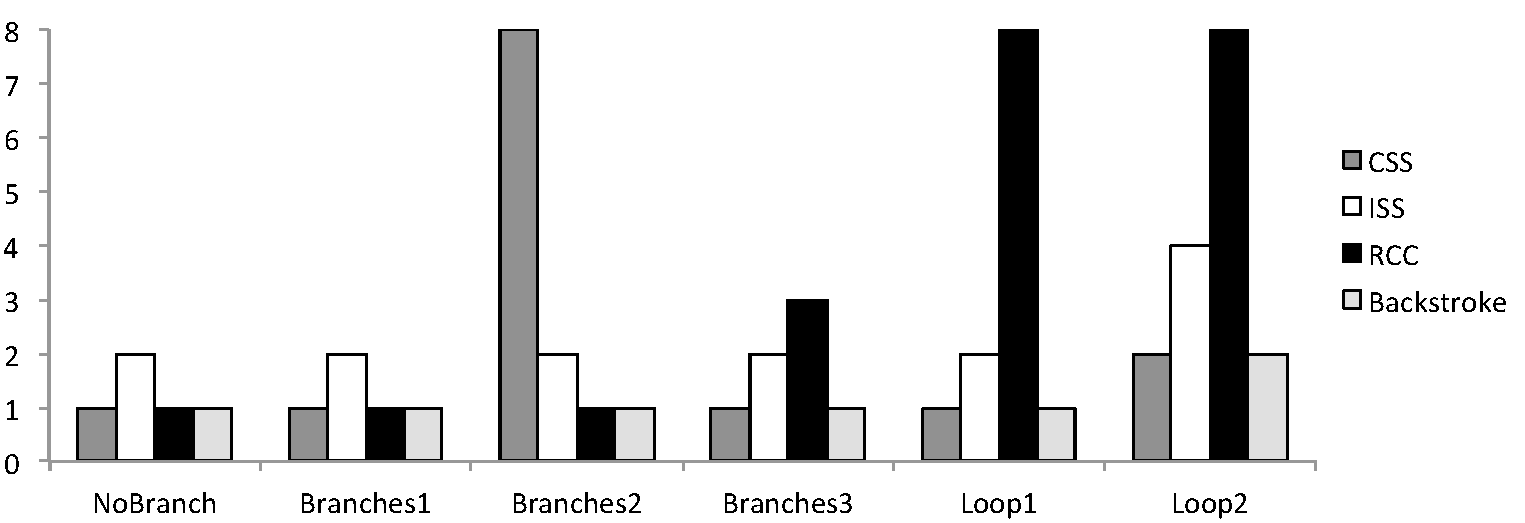
\includegraphics[width=\FigSize]{figures1/chart1.pdf}
\caption{Maximum memory usage of \Asn}
%\label{fig:code_example}
\end{subfigure}
\\
\begin{subfigure}{\textwidth}
\centering
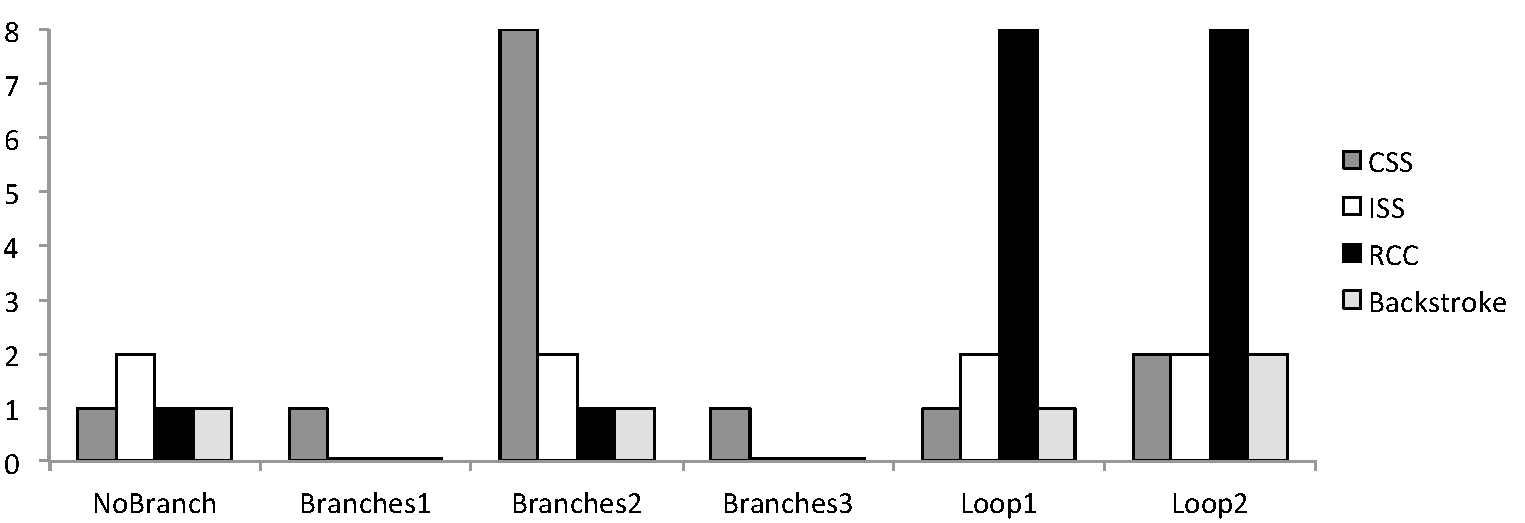
\includegraphics[width=\FigSize]{figures1/chart2.pdf}
\caption{Minimum memory usage of \Asn}
\end{subfigure}
\\
\begin{subfigure}{\textwidth}
\centering
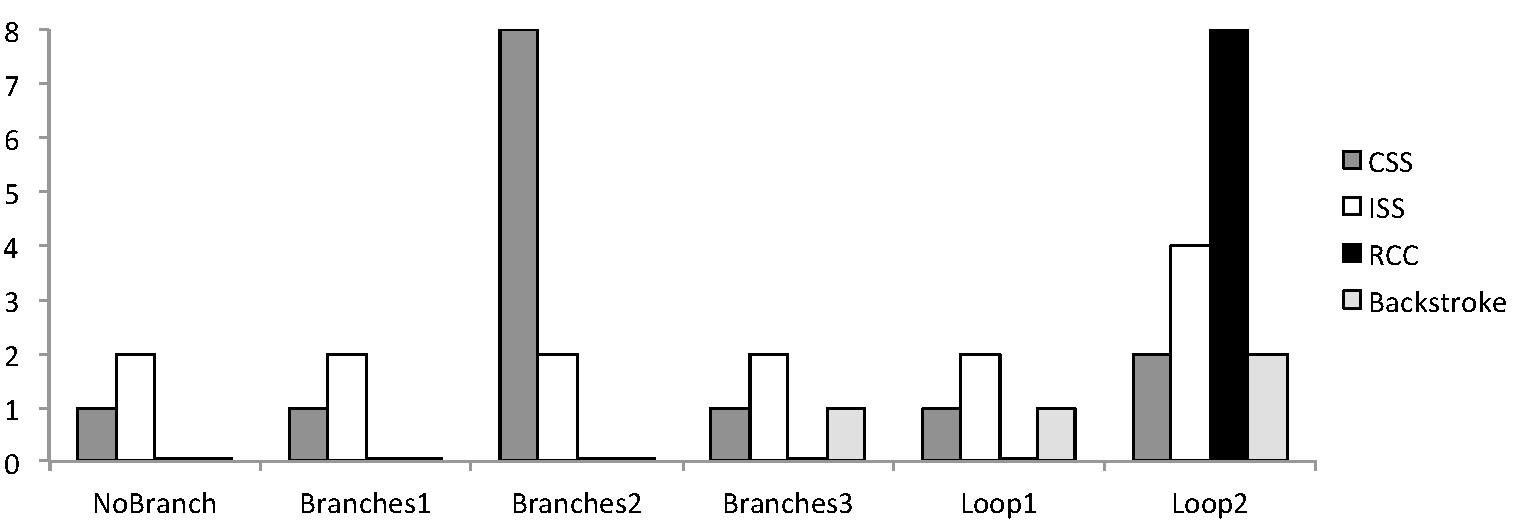
\includegraphics[width=\FigSize]{figures1/chart3.pdf}
\caption{Maximum memory usage of \Inc}
\end{subfigure}
\\
\begin{subfigure}{\textwidth}
\centering
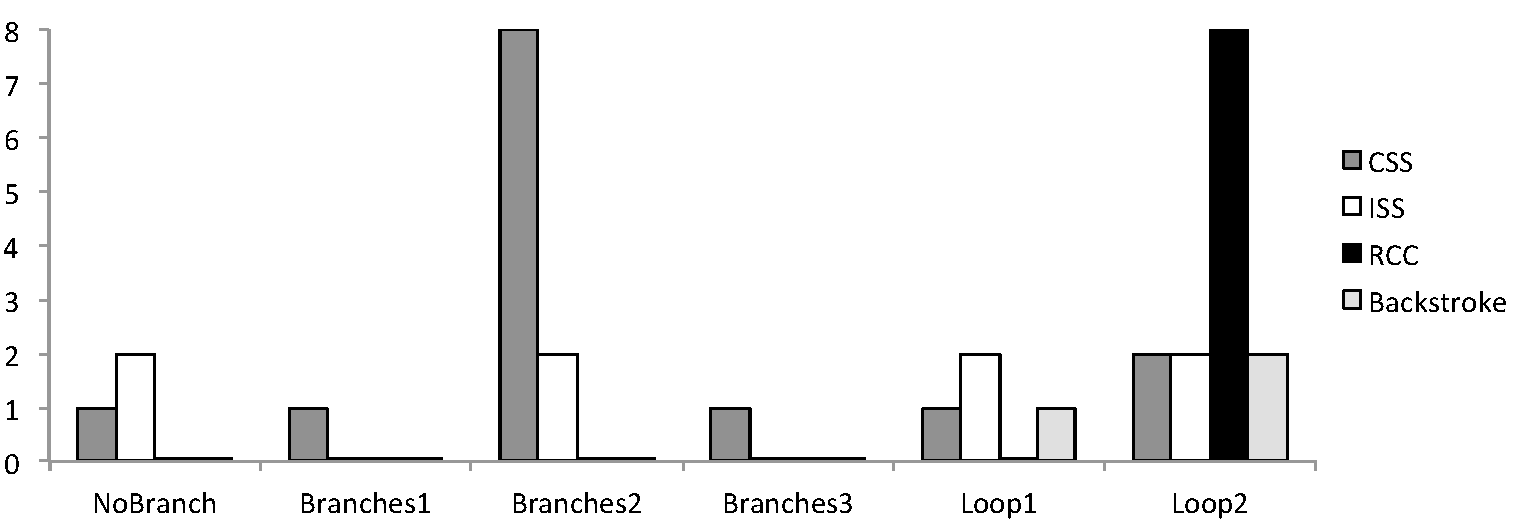
\includegraphics[width=\FigSize]{figures1/chart4.pdf}
\caption{Minimum memory usage of \Inc}
\end{subfigure}

\caption{Experiment results}
\label{fig:charts}
\end{figure}

From comparing the results from Figure \ref{fig:charts} (a)(b) and (c)(d), it is clear that the reverse execution approaches can save much memory. 
But the amount of benefit from reverse execution is determined by the number of opportunities for reverse computation. 
For programs that do not have many lossless operations such as \texttt{++} and \texttt{+=}, state saving still plays an important role in their inversions.

We must be very cautious when reversing a loop. If the loop solution is applied, we have to determine if storing control flow information is worth it or not.
The result of \Loopb from \RCC shows that if the number of iterations is large, storing control flows is not good idea. 
Saving state inside a loop normally is not a wise choice, as the result of \Loopa+ \Asn from \RCC show.




%Table 1 shows three examples, each including an original function and its generated forward and reverse function from our algorithm. For all of them, both \texttt{a} and \texttt{b} are target variables. The \texttt{cond1} and \texttt{cond2} are predicates whose content we don't care. In the first function \texttt{foo1()}, \texttt{a} is modified either \texttt{cond1} or \texttt{cond2} is true. If \texttt{cond1} and \texttt{cond2} are both true, it is not necessary to store \texttt{a} twice. Therefore, in the forward function, when \texttt{cond2} is true, we check if \texttt{a} is once stored or not to avoid multiple stores for the same value. This is exactly the same as incremental state saving, which is the best strategy here. The second function \texttt{foo2()} contains unstructured code.  The restoration of \texttt{a} and \texttt{b} does not need any state saving.  The function \texttt{foo3()} has a loop with an early exit. 

\begin{comment}

\begin{table}
\begin{center}
\small
\begin{tabular}{| m{3cm} | m{4.2cm} | m{4.2cm} |}
  \hline
  Original function & Forward function & Reverse function \\
  \hline \hline 
\begin{verbatim}
void foo1() {
  if (cond1)
    a = 0;
  if (cond2)
    a = 1;
} 
\end{verbatim}
  & 
\begin{verbatim}
void foo1_forward() {
  int bitvec = 0;
  if (cond1) {
    bitvec |= 2;
    store(a);
    a = 0;
  }
  if (cond2) {
    bitvec |= 1;
    if (bitvec & 3 == 1)
      store(a);
    a = 1;
  }
  store(bitvec);
} 
\end{verbatim}
   &
\begin{verbatim}
void foo1_reverse() {
  int bitvec;
  restore(bitvec);
  
  if (bitvec & 3 == 1)
    restore(a);
  else {
    if (bitvec & 2 == 2)
      restore(a);
  }
} 
\end{verbatim} 
\\
  \hline    
\begin{verbatim}
void foo2() {
  if (cond1) {
    ++a;
    if (cond2)
      goto L;
  }
  else
L:  ++b;
}
\end{verbatim}
&
\begin{verbatim}
void foo2_forward() {
  int bitvec = 0;
  if (cond1) {
    bitvec |= 2;
    ++a;
    if (cond2) {
      bitvec |= 1;
      goto L;
    }
  }
  else
L:  ++b;
  store(bitvec);
}
\end{verbatim}
&
\begin{verbatim}
void foo2_reverse() {
  int bitvec;
  restore(bitvec);
  
  if (bitvec & 2 == 2)
    --a;
  if (bitvec & 3 == 3 ||
      bitvec & 2 == 0)
    --b;
} 
\end{verbatim}
\\
  \hline    
\begin{verbatim}
void foo3() {
  while (cond1) {
    ++a;
    if (cond2)
        return;
    ++b;
  }
}
\end{verbatim}
&
\begin{verbatim}
void foo3_forward() {
  int bitvec = 0, k = 0;
  while (cond1) {
    ++a;
    if (cond2) {
      bitvec |= 1;
      return;
    }
    ++b;
    ++k;
  }
  store(k);
  store(bitvec);
}
\end{verbatim}
&
\begin{verbatim}
void foo3_reverse() {
  int bitvec = 0, k = 0;
  restore(bitvec);
  restore(k);
  
  if (bitvec & 1 == 1)
    --a;
  while (k--) {
    --b;
    --a;
  }
}
\end{verbatim}
\\
\hline
\end{tabular}
\end{center}
\caption{Three examples with generated forward and reverse functions.}
\end{table}

\end{comment}

%\subsection{Function Calls}
%For input only parameters of a function, if it is needed by the reverse function, it can be stored either by caller or by callee. Saving by caller may provide several ways to recover that value, and saving by callee may save that value conditionally.





